\section{លំហាត់ប៉ារ៉ាបូល}
%
\begin{enumerate}
  \item ចូរគូសប៉ារ៉ាបូលដែលមានកំណុំ និងបន្ទាត់ប្រាប់ទិសដូចខាងក្រោម៖
  \begin{Enumerate}(2)
    \item $ F(1,0) $ និង $ (\Delta):x=-1 $
    \item $ F(-1,0) $ និង $ (\Delta):x=1 $
    \item $ F(2,1) $ និង $ (\Delta):x=0 $
    \item $ F(4,2) $ និង $ (\Delta):x=2 $
    \item $ F(-3,1) $ និង $ (\Delta):x=-2 $
    \item $ F(0,2) $ និង $ (\Delta):x=1 $
  \end{Enumerate}
  %
   \item ចូរគូសប៉ារ៉ាបូលដែលមានកំណុំ និងបន្ទាត់ប្រាប់ទិសដូចខាងក្រោម៖
    \begin{Enumerate}(2)
      \item $ F(0,1) $ និង $ (\Delta):y=-1 $
      \item $ F(0,-1) $ និង $ (\Delta):y=1 $
      \item $ F(2,2) $ និង $ (\Delta):y=0 $
      \item $ F(-1,0) $ និង $ (\Delta):y=2 $
      \item $ F(1,2) $ និង $ (\Delta):y=-2 $
      \item $ F(0,1) $ និង $ (\Delta):y=2 $
    \end{Enumerate}
    %
	\item សរសេរសមីការស្តង់ដានៃប៉ារ៉ាបូល $ (P) $ ដែលមានកំពូលត្រង់ចំណុច $ V(h,k) $ និងមានបន្ទាត់ប្រាប់ទិស $ (\Delta):y=k-p $ ខាងក្រោម៖
	\begin{Enumerate}(2)
		\item $ V(1,2) $ និង $ (\Delta):y=3 $
		\item $ V(1,0) $ និង $ (\Delta):y=2 $
		\item $ V(0,-1) $ និង $ (\Delta):y=2 $
		\item $ V(-1,-2) $ និង $ (\Delta):y=0 $
		\item $ V(2,4) $ និង $ (\Delta):y=1 $
		\item $ V(3,3) $ និង $ (\Delta):y=-2 $
	\end{Enumerate}
	%
	\item សរសេរសមីការស្តង់ដានៃប៉ារ៉ាបូល $ (P) $ ដែលមានកំពូលត្រង់ចំណុច $ V(h,k) $ និងមានបន្ទាត់ប្រាប់ទិស $ (\Delta):x=h-p $ ខាងក្រោម៖
	\begin{Enumerate}(2)
		\item $ V(-1,1) $ និង $ (\Delta):x=1 $
		\item $ V(0,2) $ និង $ (\Delta):x=2 $
		\item $ V(-2,0) $ និង $ (\Delta):x=0 $
		\item $ V(3,2) $ និង $ (\Delta):x=-1 $
		\item $ V(2,4) $ និង $ (\Delta):x=-2 $
		\item $ V(1,3) $ និង $ (\Delta):x=-3 $
	\end{Enumerate}
	%
	\item សរសេរសមីការស្តង់ដានៃប៉ារ៉ាបូល $ (P) $ ដែលមានកំណុំត្រង់ចំណុច $ F(h,k+p) $ និងមានបន្ទាត់ប្រាប់ទិស $ (\Delta):y=k-p $ ខាងក្រោម៖
	\begin{Enumerate}(2)
		\item $ F(2,1) $ និង $ (\Delta):y=3 $
		\item $ F(-2,0) $ និង $ (\Delta):y=-4 $
		\item $ F(3,4) $ និង $ (\Delta):y=-2 $
		\item $ F(3,-5) $ និង $ (\Delta):y=3 $
		\item $ F(0,-4) $ និង $ (\Delta):y=-6 $
		\item $ F(-3,3) $ និង $ (\Delta):y=9 $
	\end{Enumerate}
	%
	\item សរសេរសមីការស្តង់ដានៃប៉ារ៉ាបូល $ (P) $ ដែលមានកំណុំត្រង់ចំណុច $ F(h+p,k) $ និងមានបន្ទាត់ប្រាប់ទិស $ (\Delta):x=h-p $ ខាងក្រោម៖
	\begin{Enumerate}(2)
		\item $ F(2,1) $ និង $ (\Delta):x=0 $
		\item $ F(3,-2) $ និង $ (\Delta):x=-1 $
		\item $ F(-1,2) $ និង $ (\Delta):x=-5 $
		\item $ F(0,3) $ និង $ (\Delta):x=4 $
		\item $ F(1,4) $ និង $ (\Delta):x=5 $
		\item $ F(-2,1) $ និង $ (\Delta):x=2 $
	\end{Enumerate}
	%
	\item សរសេរសមីការស្តង់ដានៃប៉ារ៉ាបូល $ (P) $ ដែលមានកំពូលត្រង់ចំណុច $ V(h,k) $ និងកំណុំ $ F(h,k+p) $ ខាងក្រោម៖
	\begin{Enumerate}(2)
		\item $ V(2,0) $ និង $ F(2,2) $
		\item $ V(-1,3) $ និង $ F(-1,1) $
		\item $ V(1,0) $ និង $ F(1,4) $
		\item $ V(0,2) $ និង $ F(0,-1) $
		\item $ V(3,2) $ និង $ F(3,3) $
		\item $ V(-2,4) $ និង $ F(-2,-1) $
	\end{Enumerate}
	%
	\item សរសេរសមីការស្តង់ដានៃប៉ារ៉ាបូល $ (P) $ ដែលមានកំពូលត្រង់ចំណុច $ V(h,k) $ និងកំណុំ $ F(h+p,k) $ ខាងក្រោម៖
	\begin{Enumerate}(2)
		\item $ V(2,1) $ និង $ F(4,1) $
		\item $ V(0,2) $ និង $ F(-2,2) $
		\item $ V(-1,0) $ និង $ F(3,0) $
		\item $ V(4,-2) $ និង $ F(0,-2) $
		\item $ V(-2,3) $ និង $ F(4,3) $
		\item $ V(-3,-1) $ និង $ F(-5,-1) $
	\end{Enumerate}
	\item កំណត់កូអរដោនេកំពូល $ V $ កំណុំ $ F $ និងសមីការបន្ទាត់ប្រាប់ទិស $ (\Delta) $ នៃប៉ារ៉ាបូល $ (P) $ ខាងក្រោម៖
	\begin{Enumerate}(2)
		\item $ (P):x^2-2x+4y-3=0 $
		\item $ (P):y^2+2x+4y=0 $
		\item $ (P):-x^2+4x-8y+4=0 $
		\item $ (P):-y^2-4x+6y-5=0 $
		\item $ (P):-2y^2+3x-4y=0 $
		\item $ (P):2x^2+3x+4y+5=0 $
	\end{Enumerate}
	%
	\item សង់ប៉ារ៉ាបូល $ (P) $ និងបន្ទាត់ប្រាប់ទិស $ (\Delta) $ ក្នុងតម្រុយតែមួយ៖
	\begin{Enumerate}(2)
		\item $ (P):(x-1)^2=4(1)(y-1) $
		\item $ (P):(y-1)^2=4(1)(x+2) $
		\item $ (P):(x+1)^2=4(-1)(y-2) $
		\item $ (P):y^2=2x $
		\item $ (P):x^2=4y $
		\item $ (P):y^2+4x+2y-7=0 $
	\end{Enumerate}
	%
	\item ប៉ារ៉ាបូល $ (P) $ មួយមានកំពូល $ V(1,0) $ និងមានបន្ទាត់ប្រាប់ទិស $ (\Delta): y=1 $~។
	\begin{Enumerate}
		\item សរសេរសមីការស្តង់ដានៃប៉ារ៉ាបូល $ (P) $
		\item កំណត់កូអរដោនេកំណុំ $ F $ នៃប៉ារ៉ាបូល $ (P) $~។
	\end{Enumerate}
	\item ប៉ារ៉ាបូល $ (P) $ មួយមានកំពូល $ V(2,-3) $ និងមានបន្ទាត់ប្រាប់ទិស $ (\Delta): x=-2 $~។
	\begin{Enumerate}
		\item សរសេរសមីការស្តង់ដានៃប៉ារ៉ាបូល $ (P) $
		\item កំណត់កូអរដោនេកំណុំ $ F $ នៃប៉ារ៉ាបូល $ (P) $~។
	\end{Enumerate}
	\item ប៉ារ៉ាបូល $ (P) $ មួយមានកំពូល $ V(2,-2) $ និងមានកំណុំ $ F(2,2) $~។
	\begin{Enumerate}
		\item សរសេរសមីការស្តង់ដានៃប៉ារ៉ាបូល $ (P) $
		\item សរសេរសមីការបន្ទាត់ប្រាប់ទិស $ (\Delta) $ នៃប៉ារ៉ាបូល $ (P) $~។
	\end{Enumerate}
	\item ប៉ារ៉ាបូល $ (P) $ មួយមានកំពូល $ V(1,0) $ និងមានកំណុំ $ F(-5,0) $~។
	\begin{Enumerate}
		\item សរសេរសមីការស្តង់ដានៃប៉ារ៉ាបូល $ (P) $
		\item សរសេរសមីការបន្ទាត់ប្រាប់ទិស $ (\Delta) $ នៃប៉ារ៉ាបូល $ (P) $~។
	\end{Enumerate}
	\item ប៉ារ៉ាបូល $ (P) $ មានសមីការ $ (P): x^2-4x+4y=0 $~។
	\begin{Enumerate}
		\item សរសេរសមីការស្តង់ដានៃប៉ារ៉ាបូល $ (P) $
		\item រកកូអរដោនេកំពូល $ V $ កំណុំ $ F $ និង សមីការបន្ទាត់ប្រាប់ទិស $ (\Delta) $~។
	\end{Enumerate}
	\item ប៉ារ៉ាបូល $ (P) $ មានសមីការ $ (P): y^2+4x-6y+1=0 $~។
	\begin{Enumerate}
		\item សរសេរសមីការស្តង់ដានៃប៉ារ៉ាបូល $ (P) $
		\item រកកូអរដោនេកំពូល $ V $ កំណុំ $ F $ និង សមីការបន្ទាត់ប្រាប់ទិស $ (\Delta) $~។
	\end{Enumerate}
	%
	\item ប៉ារ៉ាបូល $ (P) $ កាត់តាមចំណុច $ (-9,3),(-4,1) $ និង $ (-1,-1) $ និងមានបន្ទាត់ប្រាប់ទិស $ (\Delta): x=1 $~។
	\begin{Enumerate}
		\item សរសេរសមីការទូទៅនៃប៉ារ៉ាបូល $ (P) $
		\item រកកូអរដោនេកំពូល $ V $ និង កូអរដោនេកំណុំ $ F $
	\end{Enumerate}
	%
	\item ប៉ារ៉ាបូល $ (P) $ កាត់តាម $ (0,3),(3,0) $ និង $ (8,5) $ ហើយមានបន្ទាត់ប្រាប់ទិស $ (\Delta) $ ស្របអ័ក្សអរដោនេ។
	\begin{Enumerate}
		\item សរសេរសមីការទូទៅនៃប៉ារ៉ាបូល $ (P) $
		\item រកកូអរដោនកំពូល $ V $ កំណុំ $ F $ និងសមីការបន្ទាត់ប្រាប់ទិស $ (\Delta) $~។
	\end{Enumerate}
	%
	\item ប៉ារ៉ាបូល $ (P) $ កាត់តាមចំណុច $ (0,0),(2,-3) $ និង $ (-4,0) $ និងមានបន្ទាត់ប្រាប់ទិស $ (\Delta) $ ស្របនឹងអ័ក្សអាប់ស៊ីស។
	\begin{Enumerate}
		\item សរសេរសមីការទូទៅនៃប៉ារ៉ាបូល $ (P) $
		\item រកកូអរដោនេកំពូល​ $ V $ កំណុំ $ F $ និងសមីការបន្ទាត់ប្រាប់ទិស $ (\Delta) $~។
	\end{Enumerate}
	%
	\item ប៉ារ៉ាបូល $ (P) $ មានកំពូល $ V(1,-4) $ ហើយកាត់អ័ក្សអាប់ស៊ីសត្រង់ $ x=-1 $ និង $ x=3 $~។
	\begin{Enumerate}
		\item សរសេរសមីការទូទៅនៃប៉ារ៉ាបូល $ (P) $
		\item រកកូអរដោនេកំណុំ និងសមីការបន្ទាត់ប្រាប់ទិស $ (\Delta) $ នៃប៉ារ៉ាបូល $ (P) $
		\item គណនាផ្ទៃក្រឡាដែលខ័ណ្ឌដោយប៉ារ៉ាបូល $ (P) $ នឹងអ័ក្សអាប់ស៊ីស។
	\end{Enumerate}
	%
	\item គេមានប៉ារ៉ាបូល $ (P): (x+2)^2=4(-1)(y-2) $ និងបន្ទាត់ $ (L):x-2y+2=0  $~។
	\begin{Enumerate}
		\item រកកូអរដោនេចំណុចប្រសព្វរវាងប៉ារ៉ាបូល $ (P) $ និងបន្ទាត់ $ (L) $
		\item សិក្សាទីតាំងប៉ារ៉ាបូល $ (P) $ ធៀបនឹងបន្ទាត់ $ (L) $ លើចន្លោះ $ (-6,0) $
		\item គណនាផ្ទៃក្រឡាដែលខ័ណ្ឌដោយប៉ារ៉ាបូល $ (P) $ និងបន្ទាត់ $ (L) $
		\item សង់ប៉ារ៉ាបូល $ (P) $ និងបន្ទាត់ $ (L) $ ក្នុងតម្រុយតែមួយ~។
	\end{Enumerate}
	\item គេមានប៉ារ៉ាបូល $ (P): (y-1)^2=4(1)(x+2) $ បន្ទាត់ $ (M):y=-1 $ និងបន្ទាត់ $ (L):2x+y-1=0  $~។
	\begin{Enumerate}
		\item រកកូអរដោនេចំណុចប្រសព្វរវាងប៉ារ៉ាបូល $ (P) $ និងបន្ទាត់ $ (L) $
		\item សិក្សាទីតាំងប៉ារ៉ាបូល $ (P) $ ធៀបនឹងបន្ទាត់ $ (L) $ លើចន្លោះ $ (-6,0) $
		\item សង់ប៉ារ៉ាបូល $ (P) $ បន្ទាត់ $ (L) $ និងបន្ទាត់ $ (M) $ ក្នុងតម្រុយតែមួយ
		\item គណនាផ្ទៃក្រឡាដែលខ័ណ្ឌដោយប៉ារ៉ាបូល $ (P) $ បន្ទាត់ $ (L) $ និង $ (M) $~។
	\end{Enumerate}
	%
	\item គេមានប៉ារ៉ាបូល $ (P):y=x^2 $ និង $ (P'):x=y^2 $~។
	\begin{Enumerate}
		\item សង់ប៉ារ៉ាបូល $ (P) $ និង $ (P') $ ក្នុងតម្រុយតែមួយ
		\item រកកូអរដោនេចំណុចប្រសព្វរវាងប៉ារ៉ាបូលទាំងពីរ
		\item គណនាផ្ទៃក្រឡាដែលខ័ណ្ឌដោយប៉ារ៉ាបូលទាំងពីរ
	\end{Enumerate}
	%
	\item គេមានប៉ារ៉ាបូល $ (P): -x^2+4x+y=0 $ និង $ (P'):-y^2+x+4y=0 $ ដែលមានក្រាបដូចរូប។
	%
	\begin{figure}[H]
		\centering
		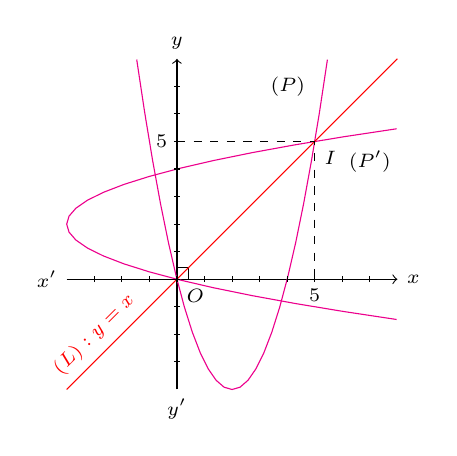
\begin{tikzpicture}[x=.35cm,y=.35cm,font=\scriptsize]
			\coordinate(O)at(0,0);
			\coordinate(X')at(-4,0);
			\coordinate(X)at(8,0);
			\coordinate(Y')at(0,-4);
			\coordinate(Y)at(0,8);
			\coordinate(I)at(5,5);
			\coordinate(Lb)at(-4,-4);
			\coordinate(Le)at(8,8);
			\draw[->](X')node[left]{$ x' $}--(X)node[right]{$ x $};
			\draw[->](Y')node[below]{$ y' $}--(Y)node[above]{$ y $};
			\draw([yshift=1ex]O)--([xshift=1ex,yshift=1ex]O)--([xshift=1ex]O);
			\draw[magenta]plot[domain=-1.46:5.46](\x,{\x*(\x-4)});
			\draw[magenta]plot[domain=-1.46:5.46]({\x*(\x-4)},\x);
			\draw[red](Lb)--node[sloped,very near start,above]{$ (L):y=x $}(Le);
			\draw[dashed](I-|Y)node[left]{$ 5 $}--(I)--(I|-X)node[below]{$ 5 $};
			\foreach\n in {-3,-2,...,7}{%
			\draw(\n,-1pt)--(\n,1pt);%
			\draw(-1pt,\n)--(1pt,\n);}
			\foreach\p in {O,I}{\node[below right]at(\p){$ \p $};}
			\node[left] at(5,7){$ (P) $};
			\node[below] at(7,5){$ (P') $};
		\end{tikzpicture}
	\end{figure}
	%
	\begin{Enumerate}
		\item បង្ហាញថាប៉ារ៉ាបូល $ (P) $ និង $ (P') $ ឆ្លុះគ្នាធៀបនឹងបន្ទាត់ពុះទីមួយ $ (L):y=x $
		\item គណនាផ្ទៃក្រឡាដែលខ័ណ្ឌដោយបន្ទាត់ $ (L) $ និងប៉ារ៉ាបូល $ (P) $
		\item គណនាផ្ទៃក្រឡា បេះដូង ដែលខ័ណ្ឌដោយប៉ារ៉ាបូល $ (P) $ និង $ (P') $~។
	\end{Enumerate}
	%
\end{enumerate}
%